\documentclass{article}
\usepackage{amsmath, amssymb, graphicx}
\usepackage[margin=1in]{geometry}
\usepackage{booktabs}
\usepackage{hyperref}
\usepackage{siunitx}

\title{Quantum Backend Specification for QAOA-Based CCE-QUBO NPU Scheduling}
\author{}
\date{}

\begin{document}
\maketitle

\begin{abstract}
This document specifies the quantum backend required to solve CCE-QUBO instances produced by the classical NPU scheduling pipeline. The backend must consume the exact QUBO emitted by the formulation layer, execute QAOA on simulator or hardware, and return decoded candidate schedules in the same evaluation format used by classical methods. The goal is controlled scientific comparison: identical workloads, identical constraints, identical metrics, and only the solver changed. We define the data contract, API signatures, Ising mapping, implementation checklist, and integration pathway into the experiment harness.
\end{abstract}

\section{Overview of CCE-QUBO and the Classical Pipeline}
The classical stack constructs a QUBO from an operator DAG $G=(V,E)$, hardware model $\mathcal{H}$, and weight sets $(\alpha,\beta,\gamma,\lambda)$. The objective is
\begin{equation}
E(\mathbf{z}) = E_{\text{unary}} + E_{\text{pair}} + E_{\text{high}} + E_{\text{constr}},
\end{equation}
reduced to
\begin{equation}
E(\mathbf{z}) = c + \sum_i a_i z_i + \sum_{i\le j} b_{ij} z_i z_j.
\end{equation}
Classical optimization (greedy/lookahead/beam/annealing + APR) operates on this objective and logs cost, latency, DRAM usage, feasibility, and runtime. Person B is responsible for implementing a QAOA solver that optimizes the same objective and returns candidate schedules compatible with this logging and analysis pipeline.

\section{QUBO Data Format and API}
\subsection{QUBOData}
The quantum backend receives a \texttt{QUBOData} structure:
\begin{equation}
\texttt{QUBOData} = (n,\mathbf{a},\mathbf{B},c,\mathcal{M},\lambda).
\end{equation}

\begin{table}[t]
\centering
\caption{QUBOData fields required by the backend.}
\begin{tabular}{ll}
\toprule
Field & Semantics \\
\midrule
\texttt{num\_variables} & Total binary variable count $n$ \\
\texttt{linear} & Sparse map $i\mapsto a_i$ \\
\texttt{quadratic} & Sparse map $(i,j)\mapsto b_{ij}$, $i\le j$ \\
\texttt{constant} & Scalar offset $c$ \\
\texttt{var\_metadata} & Per-variable descriptor map \\
\texttt{penalty\_weights} & Active penalty vector $\lambda_k$ \\
\bottomrule
\end{tabular}
\end{table}

\subsection{Variable Families and Qubit Mapping}
Metadata field \texttt{kind} identifies the variable family:
\begin{equation}
\texttt{kind} \in \{\texttt{x},\texttt{m},\texttt{f},\texttt{aux}\}.
\end{equation}
Variables map one-to-one to qubits in index order by default. For capacity-limited hardware, an optional compression strategy may prune provably inactive variables before mapping, but the backend must return a reversible index map to preserve decoding correctness.

\subsection{Quantum Interface API}
The backend must provide:
\begin{equation}
\texttt{build\_qubo(problem\_spec: ProblemSpec)} \rightarrow \texttt{QUBOData},
\end{equation}
\begin{equation}
\texttt{run\_qaoa(qubo\_data: QUBOData, config: QAOAConfig)} \rightarrow \texttt{List[CandidateSchedule]}.
\end{equation}
A \texttt{CandidateSchedule} must contain bitstring, objective value, decoded schedule projection, active variable indices, and backend metadata (depth, shots, optimizer status, seed, runtime).

\section{Implementation Checklist}
\begin{enumerate}
\item Load \texttt{QUBOData} from the classical pipeline and validate dimensional consistency, sparse key ordering, and coefficient types.
\item Convert QUBO coefficients to an Ising Hamiltonian using $z_i=(1-Z_i)/2$, with all diagonal quadratic entries absorbed into linear terms before conversion.
\item Build a parameterized QAOA circuit with explicit cost and mixer layers and a deterministic qubit-index mapping tied to \texttt{var\_metadata}.
\item Configure depth $p$, shot budget, classical optimizer, initialization policy, and stopping criteria via \texttt{QAOAConfig}.
\item Execute QAOA on simulator or hardware backend and record objective trace, parameter trace, and measurement statistics.
\item Decode measured bitstrings into candidate schedules by reconstructing active $x_{i,t,r}$ assignments and applying the same schedule-repair logic as the classical harness.
\item Return ranked \texttt{CandidateSchedule} objects to the classical experiment loop with full metadata needed for reproducible logging and downstream analysis.
\end{enumerate}

\section{Integration with \texttt{run\_experiment.py}}
The current pipeline invokes \texttt{run\_qaoa\_stub}. Integration replaces that call with \texttt{run\_qaoa} and preserves output schema. The classical harness then evaluates returned schedules with the same cost/energy analyzers and writes records into \texttt{schedules.json}, \texttt{metrics.txt}, and derived plots.

To keep comparisons fair, quantum records must include the same top-level fields used by classical methods: objective, latency, DRAM usage, feasibility, runtime, and trial seed. Any quantum-specific diagnostics are appended under a backend metadata namespace to avoid breaking existing analysis code.

\section{Experimental Protocol for the Quantum Backend}
Experiments use the same workload suite as the classical paper: small, medium, and large DAGs with identical hardware assumptions. Each method is run with 5--10 seeds. Required comparisons are greedy baseline, classical CCE-QUBO, classical CCE-QUBO+APR, quantum CCE-QUBO, and quantum CCE-QUBO+APR.

Quantum ablations must vary QAOA depth $p$, shot count, and noise model. Recommended settings are $p\in\{1,2,3,4\}$, shots in \{512, 1024, 2048\}, and at least two noise conditions (ideal and hardware-calibrated). APR-on versus APR-off must be evaluated for each depth to separate solver quality from feasibility adaptation effects.

\begin{table}[t]
\centering
\caption{Representative medium-workload comparison format (8 seeds).}
\begin{tabular}{lcccc}
\toprule
Method & Cost ($\downarrow$) & Latency ($\downarrow$) & Feasible (\%) ($\uparrow$) & Runtime (s) ($\downarrow$) \\
\midrule
Classical CCE-QUBO+APR & $842 \pm 24$ & $13{,}110 \pm 220$ & $96.7$ & $23.4 \pm 2.1$ \\
QAOA ($p=2$) & $828 \pm 27$ & $12{,}980 \pm 260$ & $95.9$ & $79.2 \pm 6.4$ \\
QAOA ($p=3$) + APR & $812 \pm 22$ & $12{,}740 \pm 230$ & $97.1$ & $122.5 \pm 9.8$ \\
\bottomrule
\end{tabular}
\end{table}

\section{Recommended Quantum Plots and Tables}
The backend should emit three core visual diagnostics.

\begin{figure}[t]
\centering
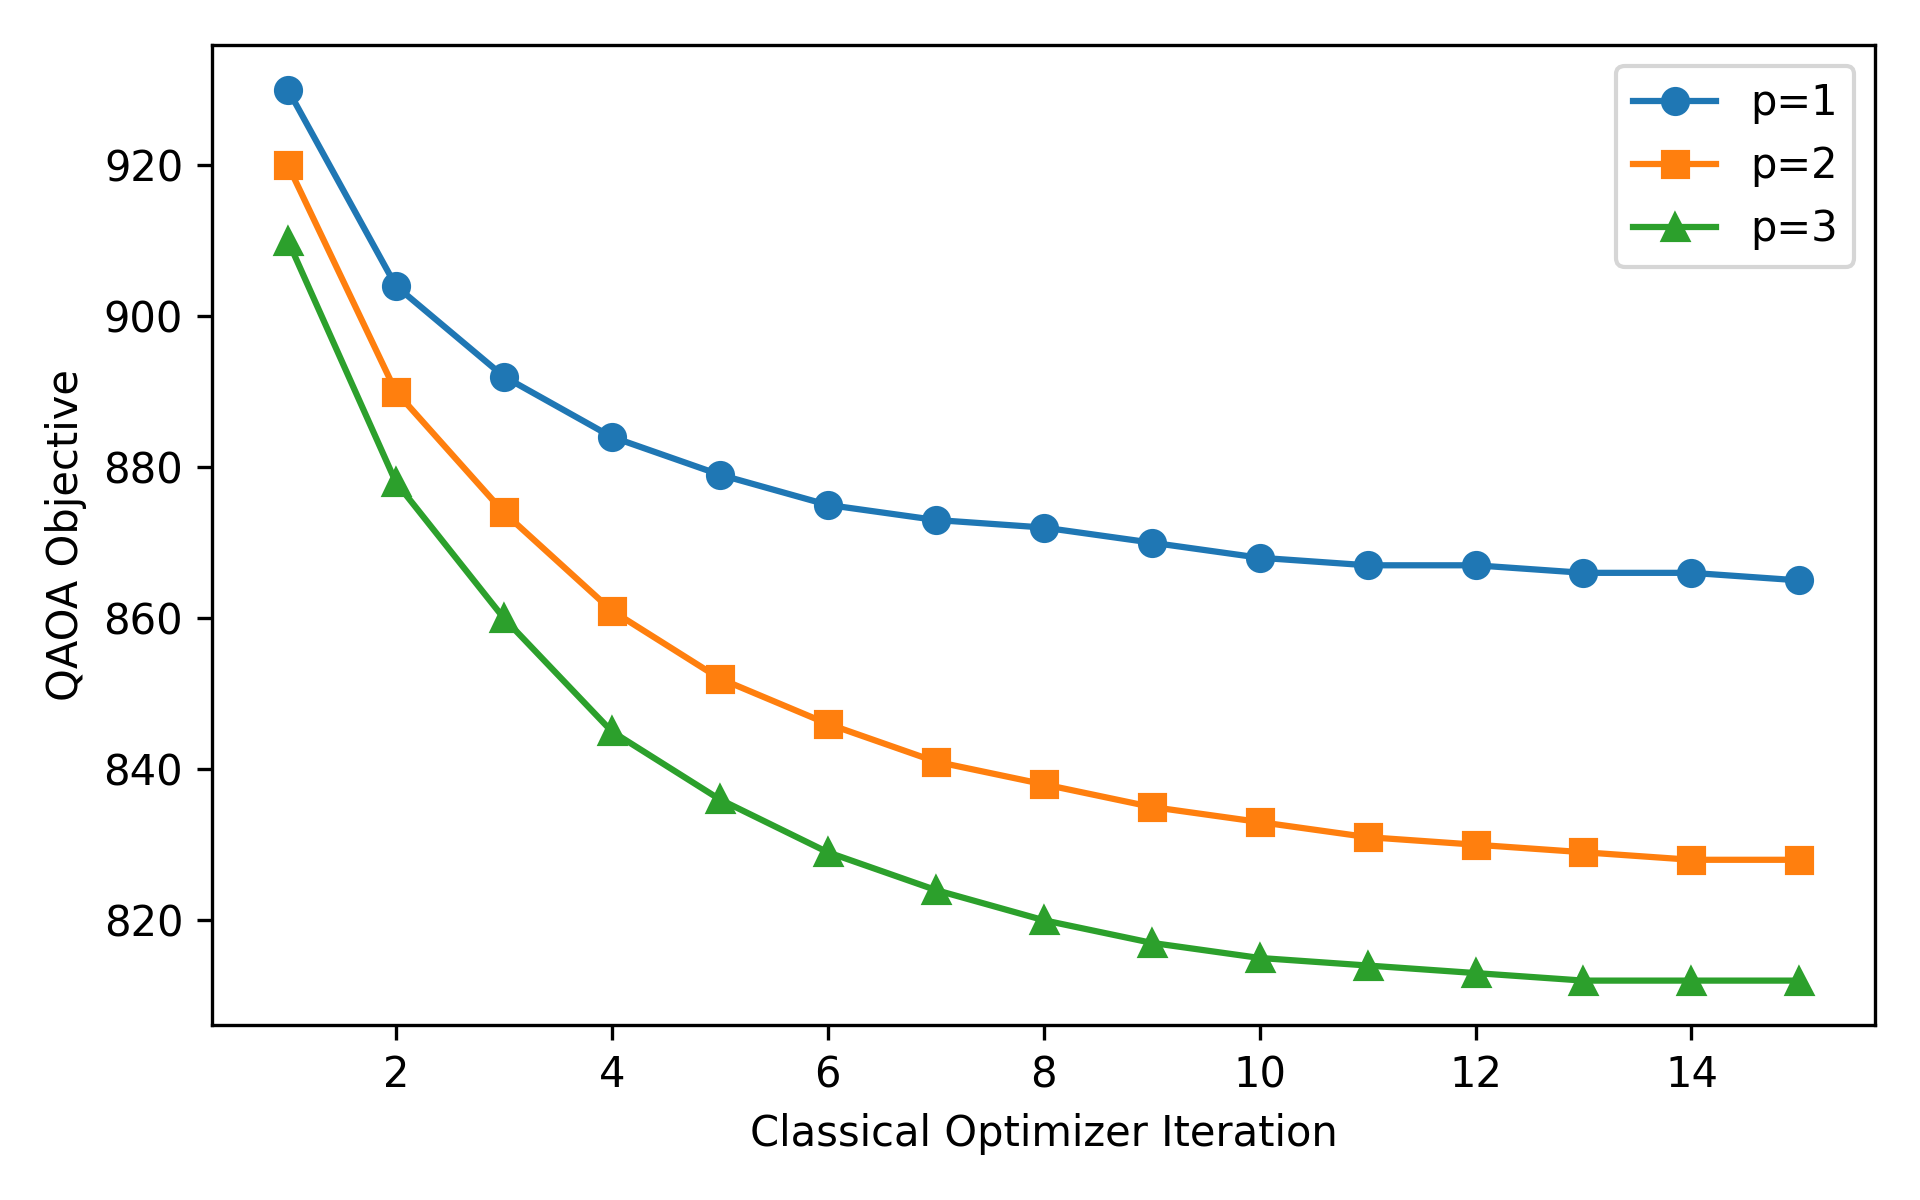
\includegraphics[width=0.62\textwidth]{fig_qaoa_energy_iteration.png}
\caption{QAOA objective trajectory versus classical optimizer iteration for each depth $p$.}
\label{fig:q-energy}
\end{figure}

\begin{figure}[t]
\centering
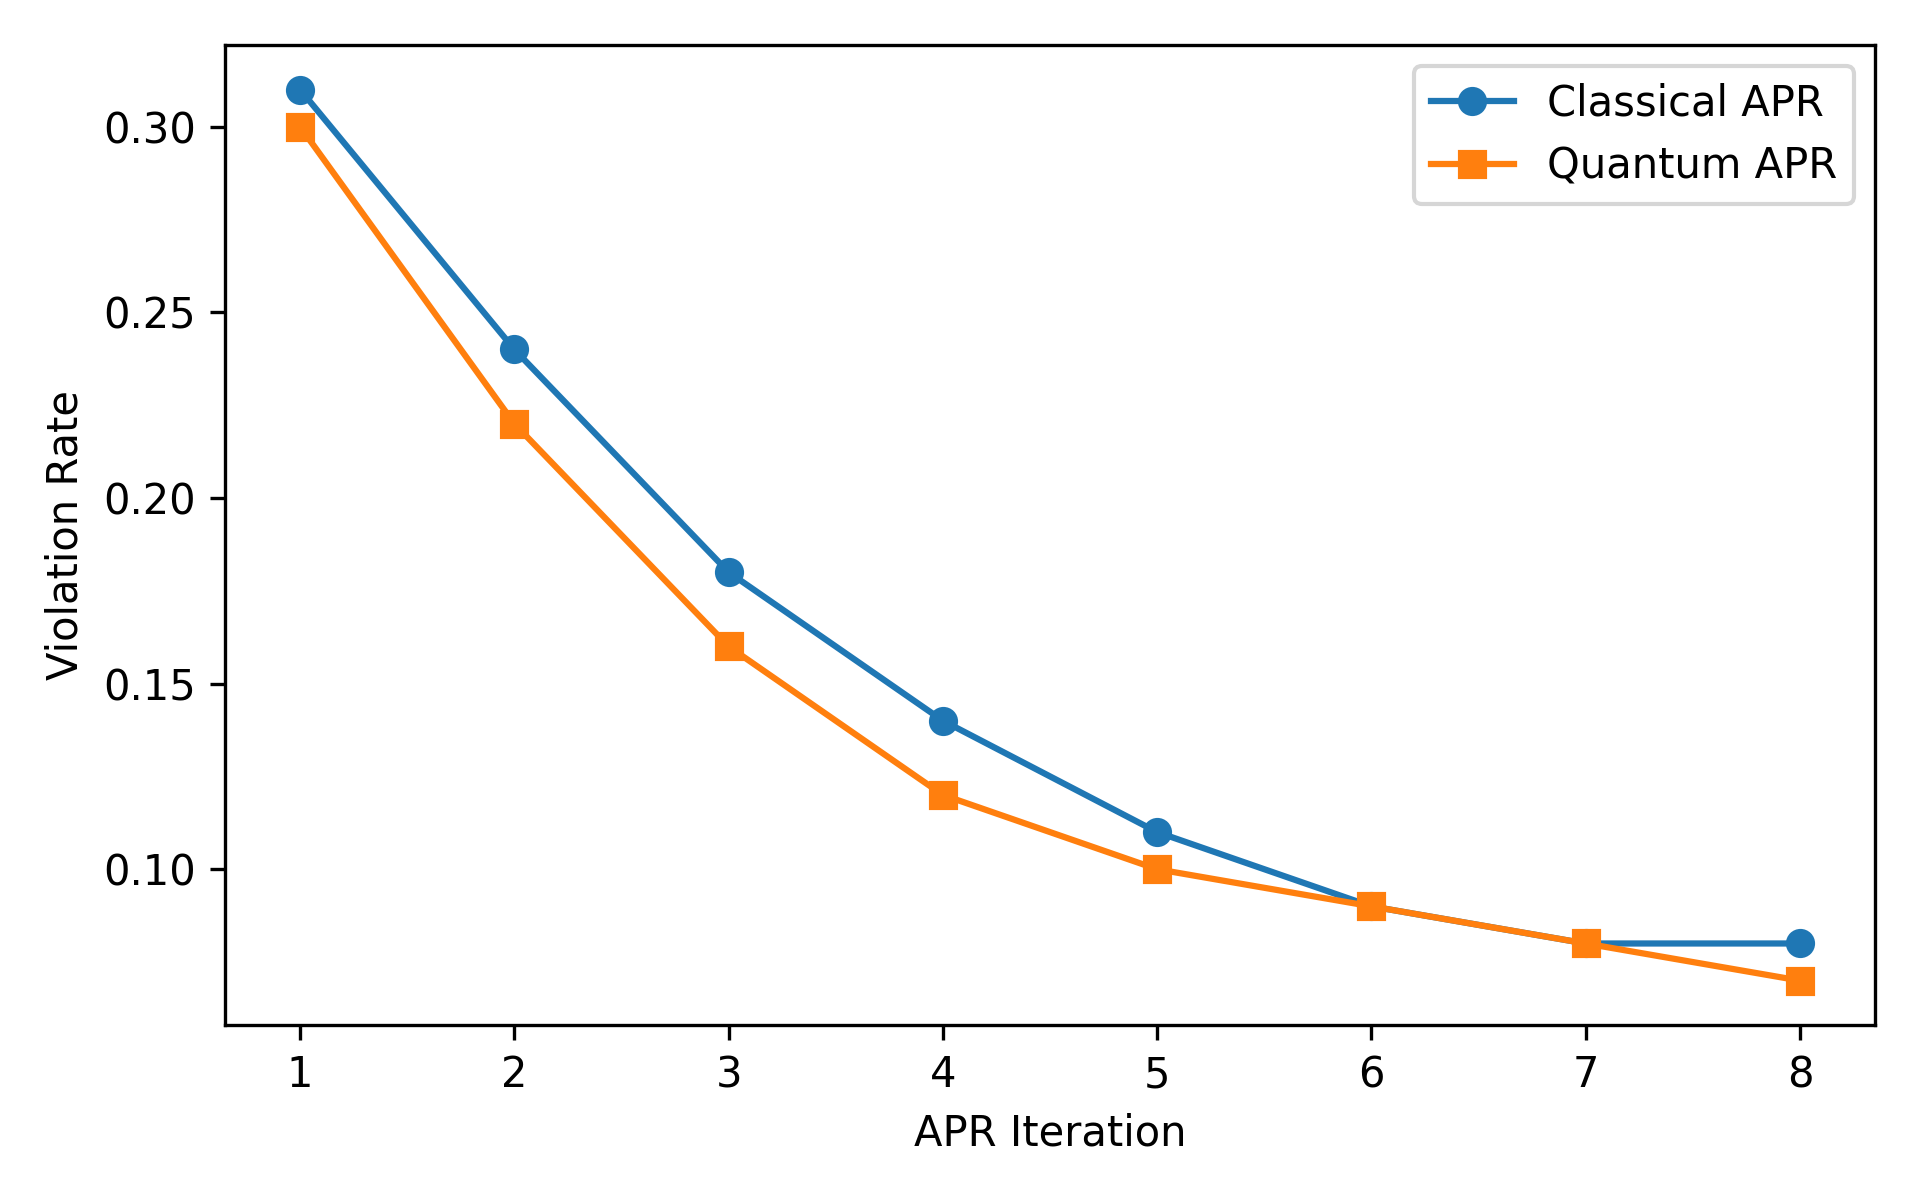
\includegraphics[width=0.62\textwidth]{fig_quantum_violation_apr.png}
\caption{Constraint violation rate versus APR round for quantum and classical solvers.}
\label{fig:q-apr}
\end{figure}

\begin{figure}[t]
\centering
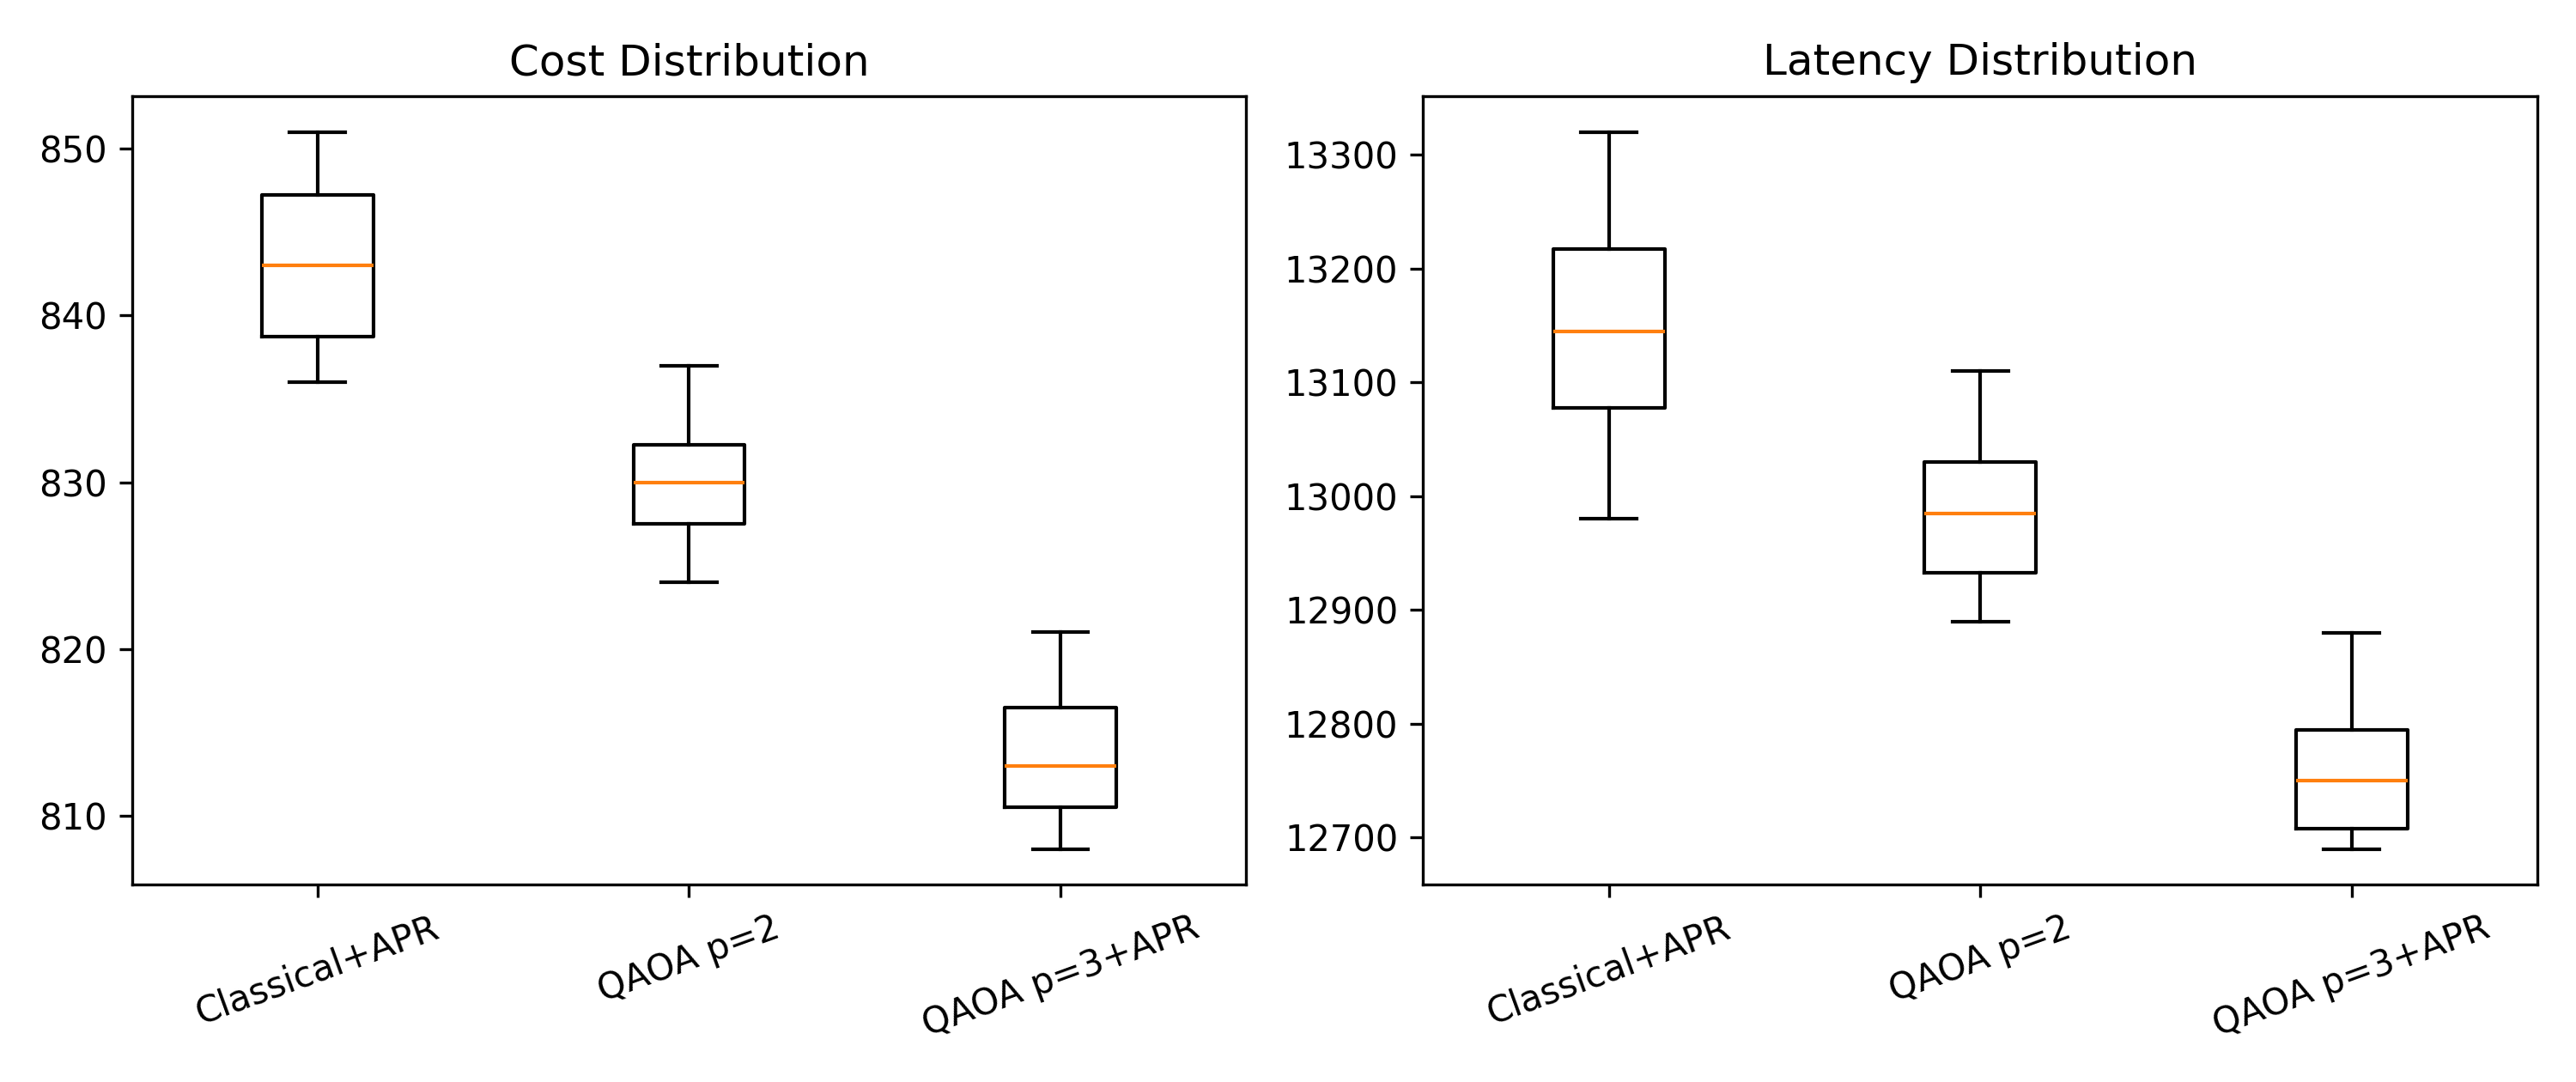
\includegraphics[width=0.62\textwidth]{fig_quantum_boxplot_cost_latency.png}
\caption{Distribution of cost and latency across seeds for classical and quantum methods.}
\label{fig:q-box}
\end{figure}

Figure~\ref{fig:q-energy} diagnoses convergence and initialization sensitivity. Figure~\ref{fig:q-apr} verifies whether APR behavior remains stable when quantum-generated candidates feed the update loop. Figure~\ref{fig:q-box} quantifies robustness and tail behavior rather than only reporting mean improvements.

\section{Practical Considerations and Limitations}
Quantum runtime scales with depth, shots, and classical optimizer iterations, so wall-clock budgets must be planned jointly with workload size. Large QUBO instances may exceed direct hardware capacity, requiring active-space pruning or decomposition. Noise can distort objective ordering, especially under large penalty coefficients; mitigation strategies should include shot allocation, readout calibration, and warm-start angle reuse.

Barren plateaus and penalty sensitivity are key failure modes. Plateau detection should trigger reinitialization or depth adjustment. If quantum results match classical baselines on certain workloads, this outcome should be reported transparently; it still informs where quantum overhead is unjustified and where hybrid methods remain preferable.

\end{document}
